\chapter{Интерфейс приложения}
\label{cha:appendix2}

\begin{figure}[h]
	\centering
	
\includegraphics[width=\textwidth]{figures/start}
	\caption{Стартовая страница веб-приложения}
	\label{fig:start}
\end{figure}

\begin{figure}[h]
	\centering
	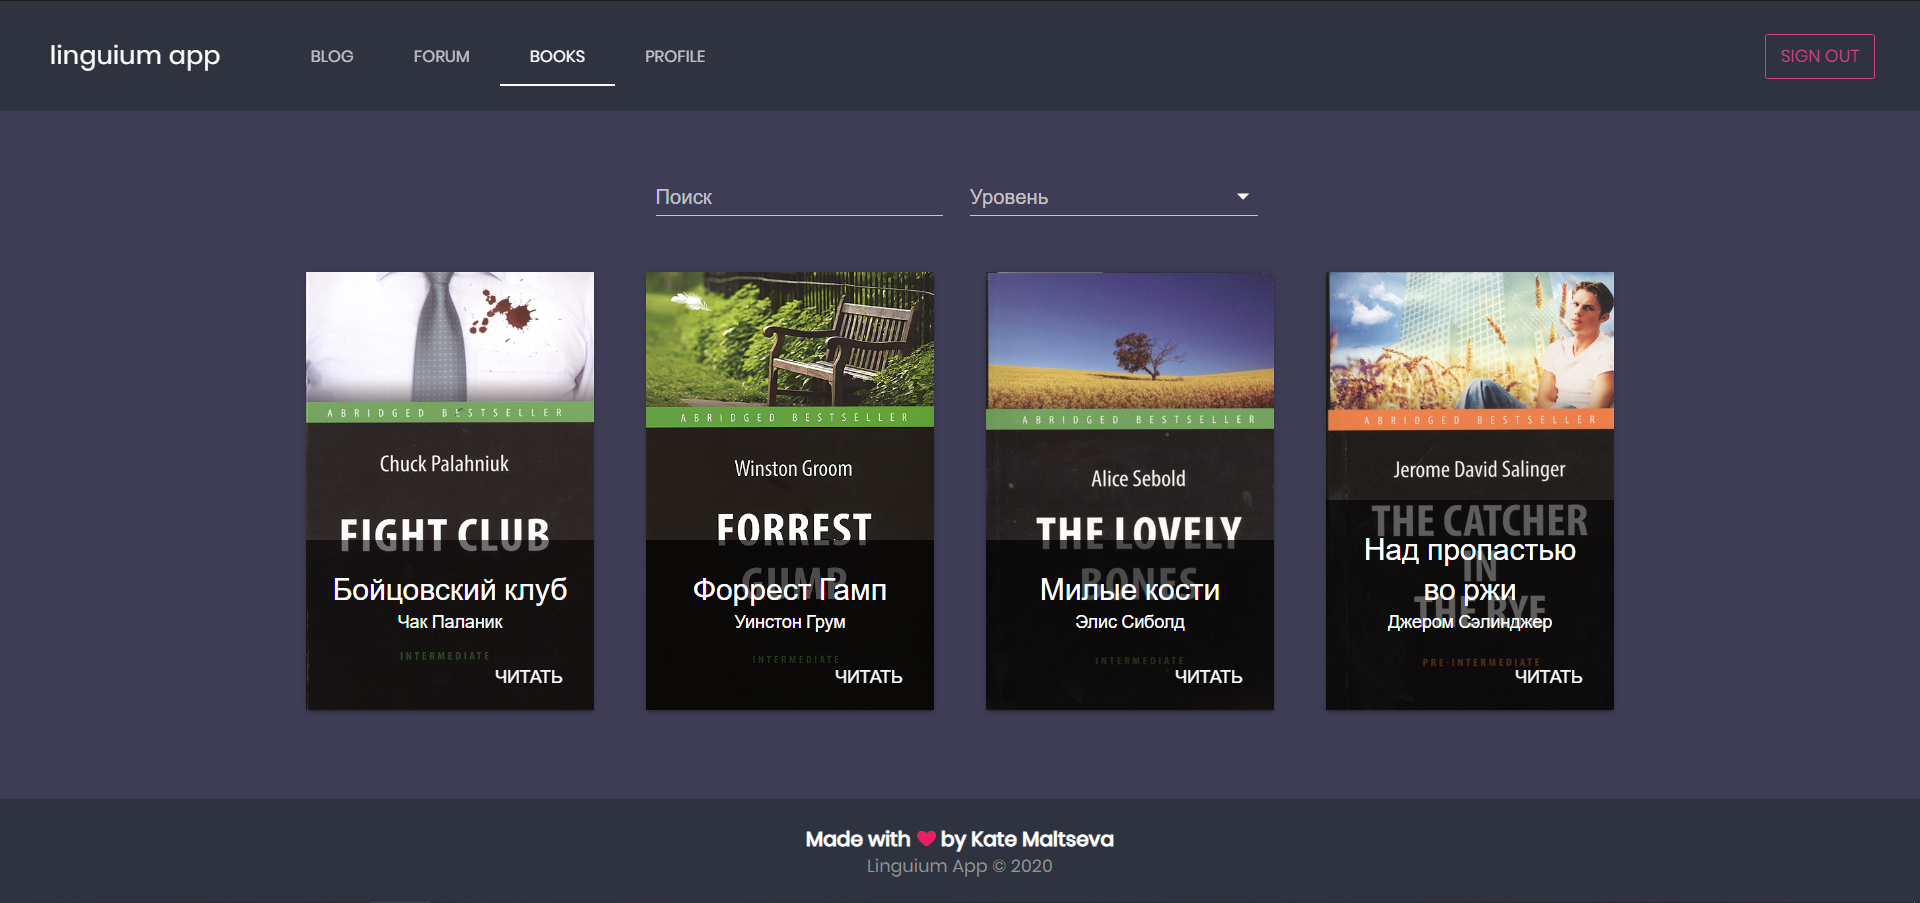
\includegraphics[width=\textwidth]{figures/booklist}
	\caption{Список доступных в приложении книг}
	\label{fig:booklist}
\end{figure}

\begin{figure}[h]
	\centering
	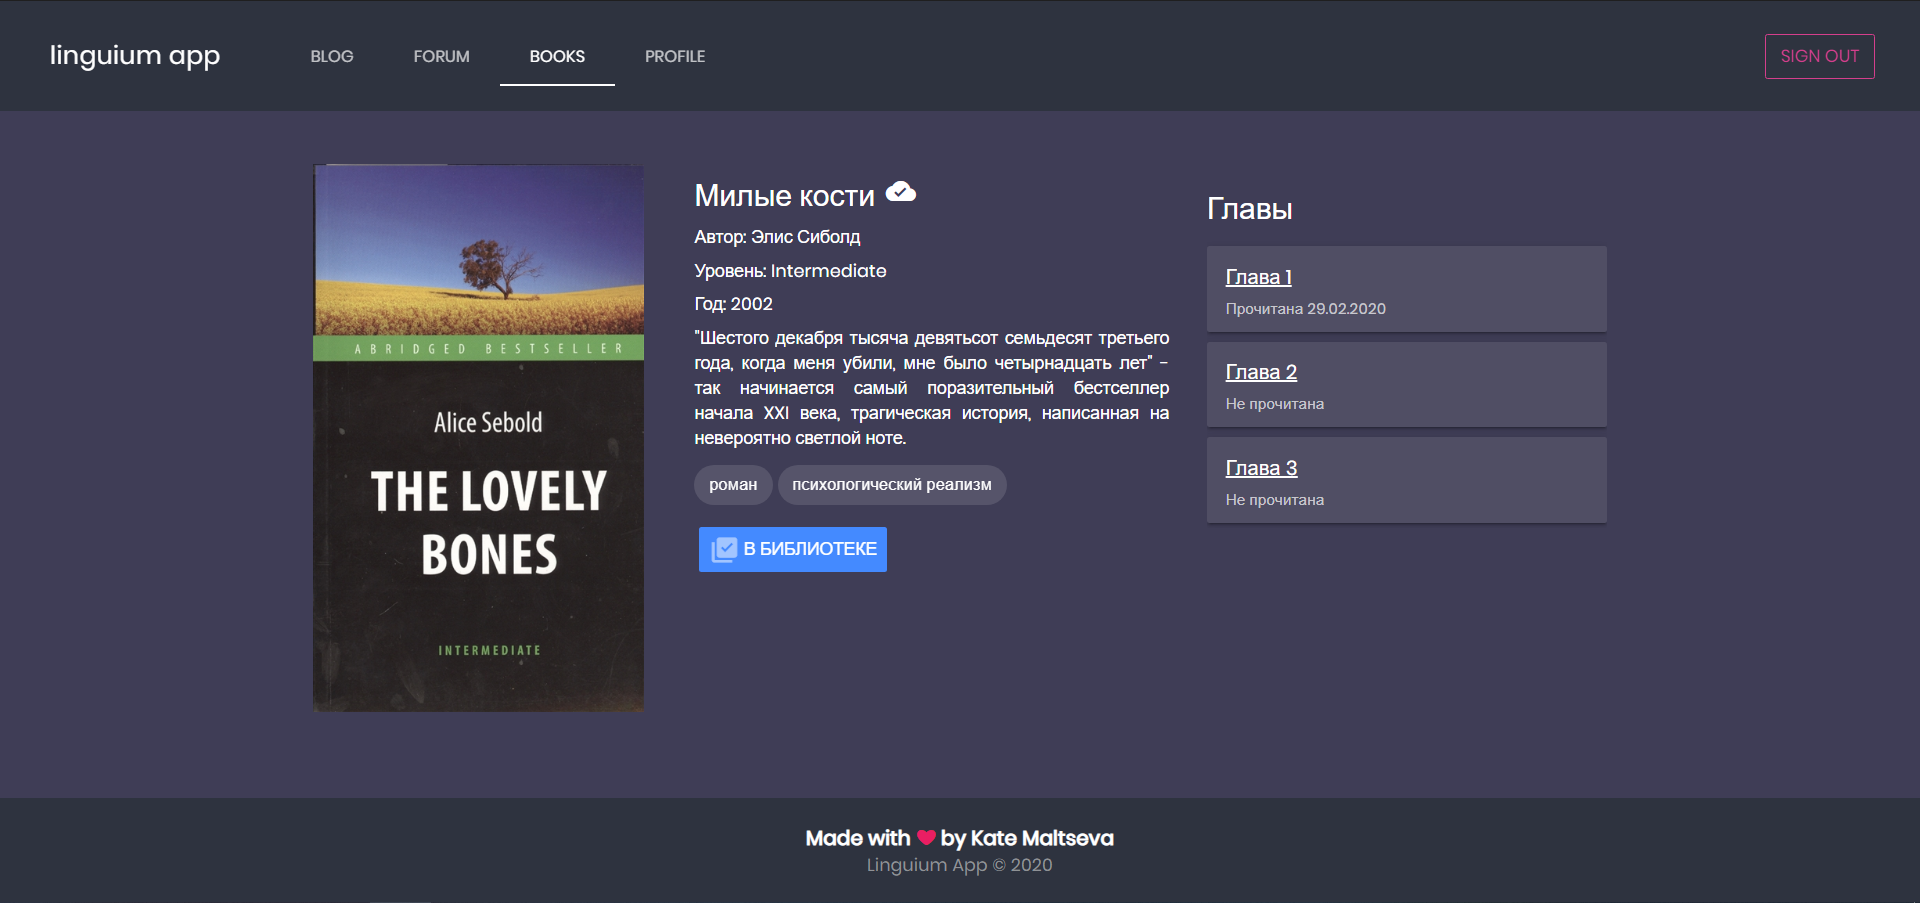
\includegraphics[width=\textwidth]{figures/bookitem}
	\caption{Информация о конкретно взятой книге и ее частях}
	\label{fig:bookitem}
\end{figure}

\begin{figure}[h]
	\centering
	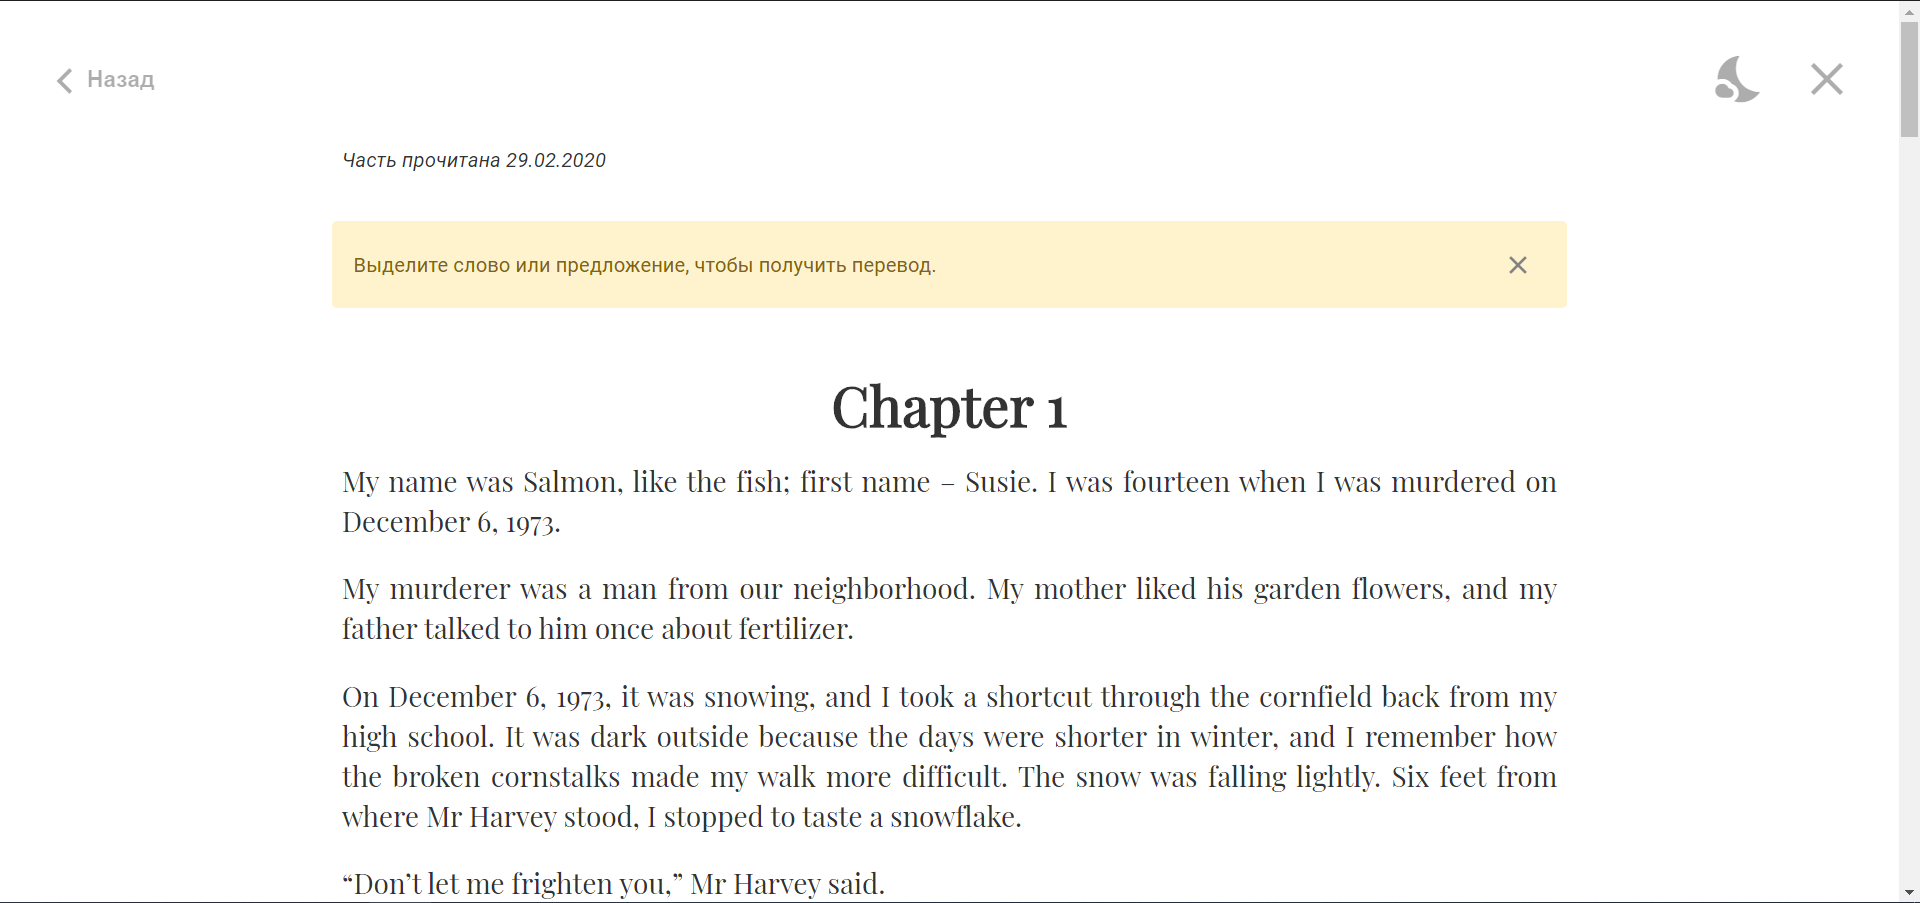
\includegraphics[width=\textwidth]{figures/reading}
	\caption{Режим чтения части книги с возможностью перевода текста и переключения темы}
	\label{fig:reading}
\end{figure}

\begin{figure}[h]
	\centering
	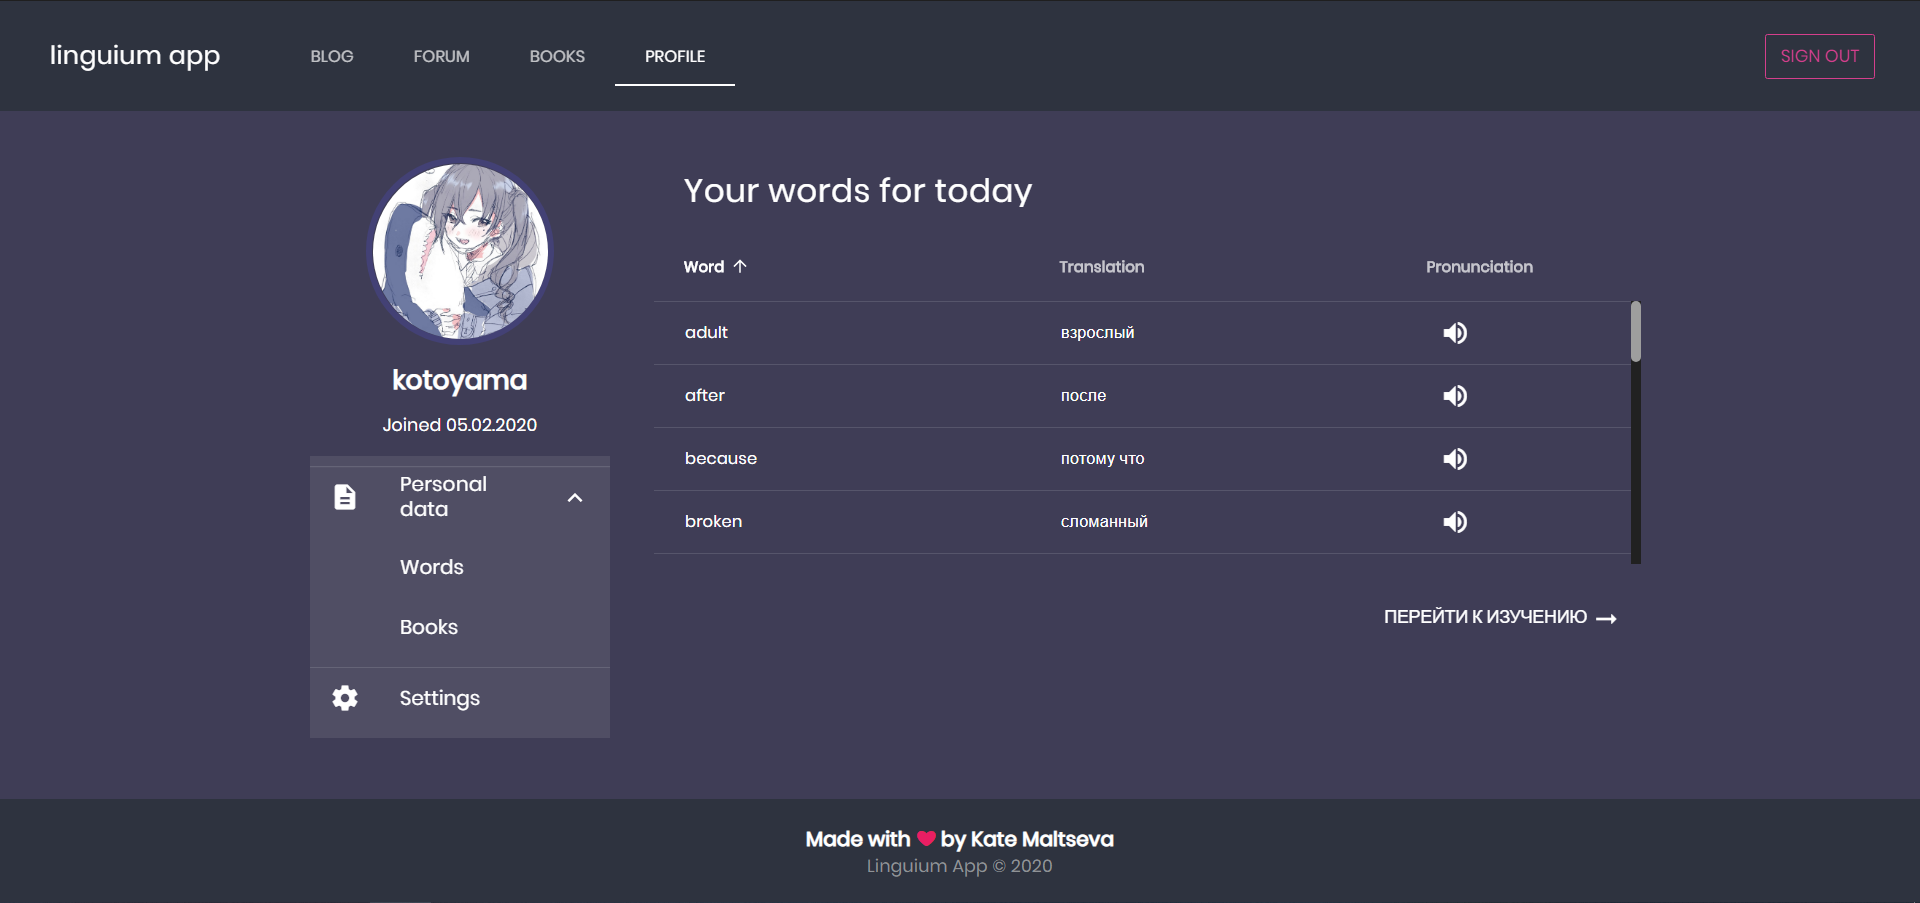
\includegraphics[width=\textwidth]{figures/profile}
	\caption{Личный кабинет пользователя со всеми его данными и возможностью настройки пользовательских данных}
	\label{fig:profile}
\end{figure}

\begin{figure}[h]
	\centering
	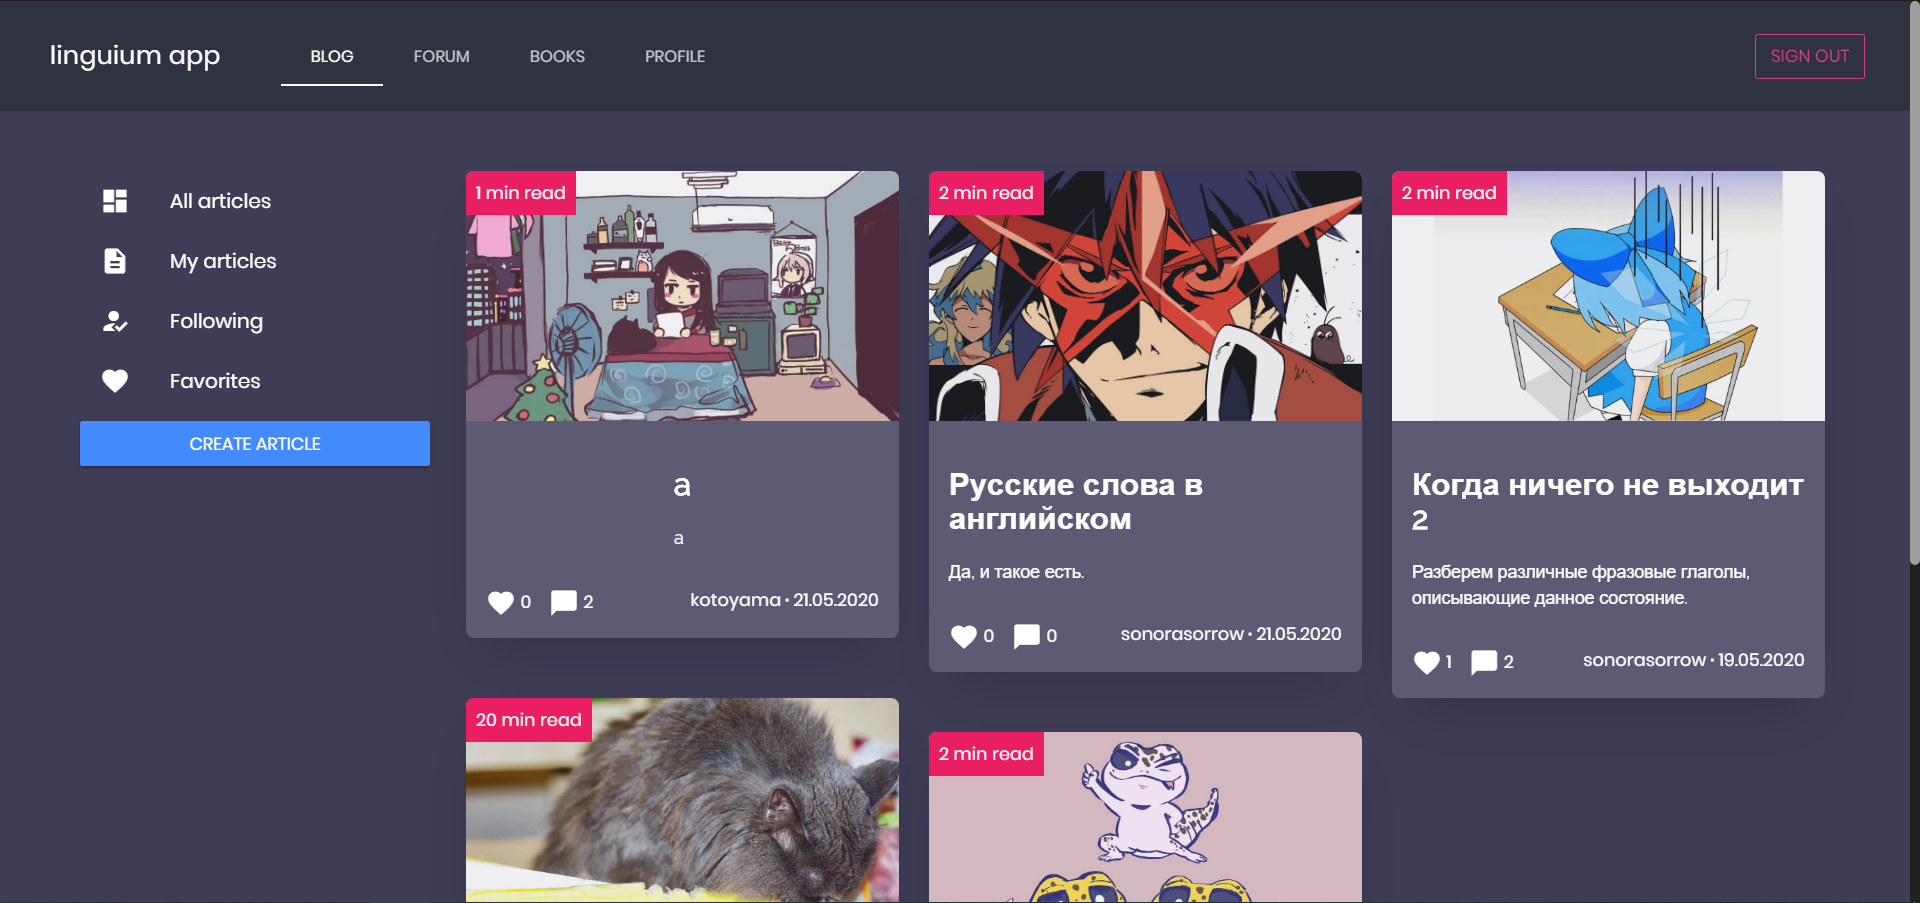
\includegraphics[width=\textwidth]{figures/articlelist}
	\caption{Список статей с возможностью их фильтрации}
	\label{fig:articlelist}
\end{figure}

\begin{figure}[h]
	\centering
	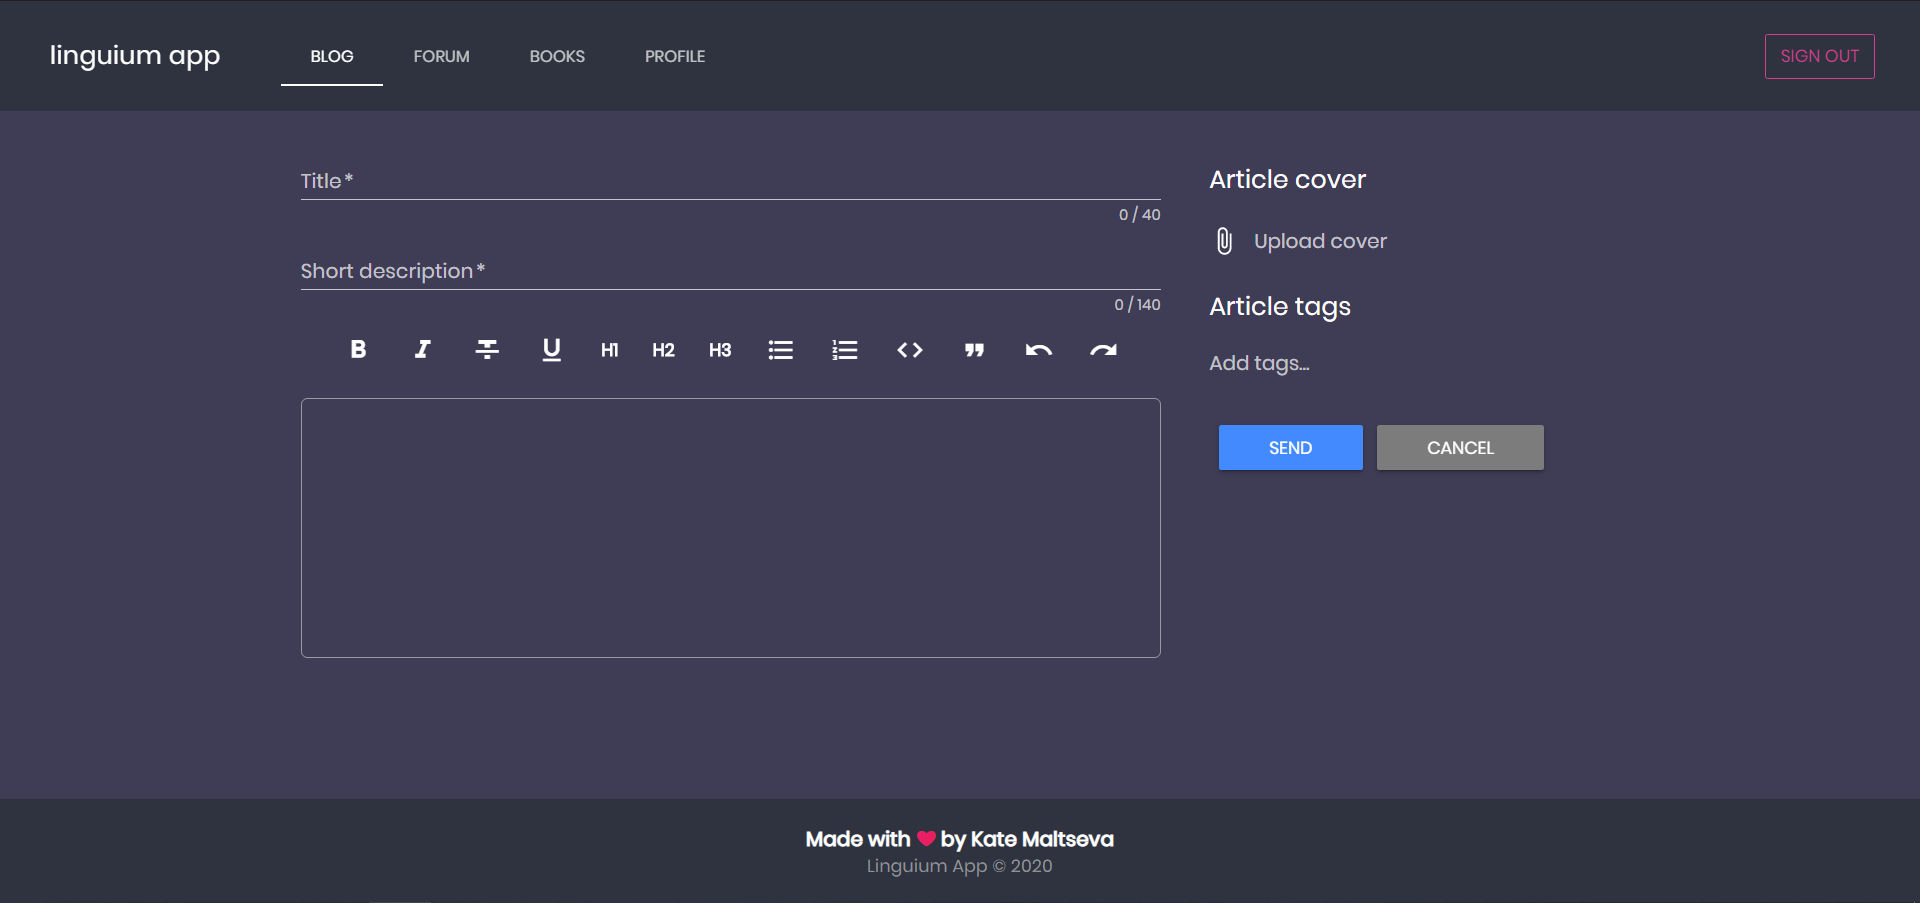
\includegraphics[width=\textwidth]{figures/createlist}
	\caption{Страница создания статьи с возможностью продвинутой верстки контента (страница для редакторования выглядит аналогичным образом)}
	\label{fig:createlist}
\end{figure}

\begin{figure}[h]
	\centering
	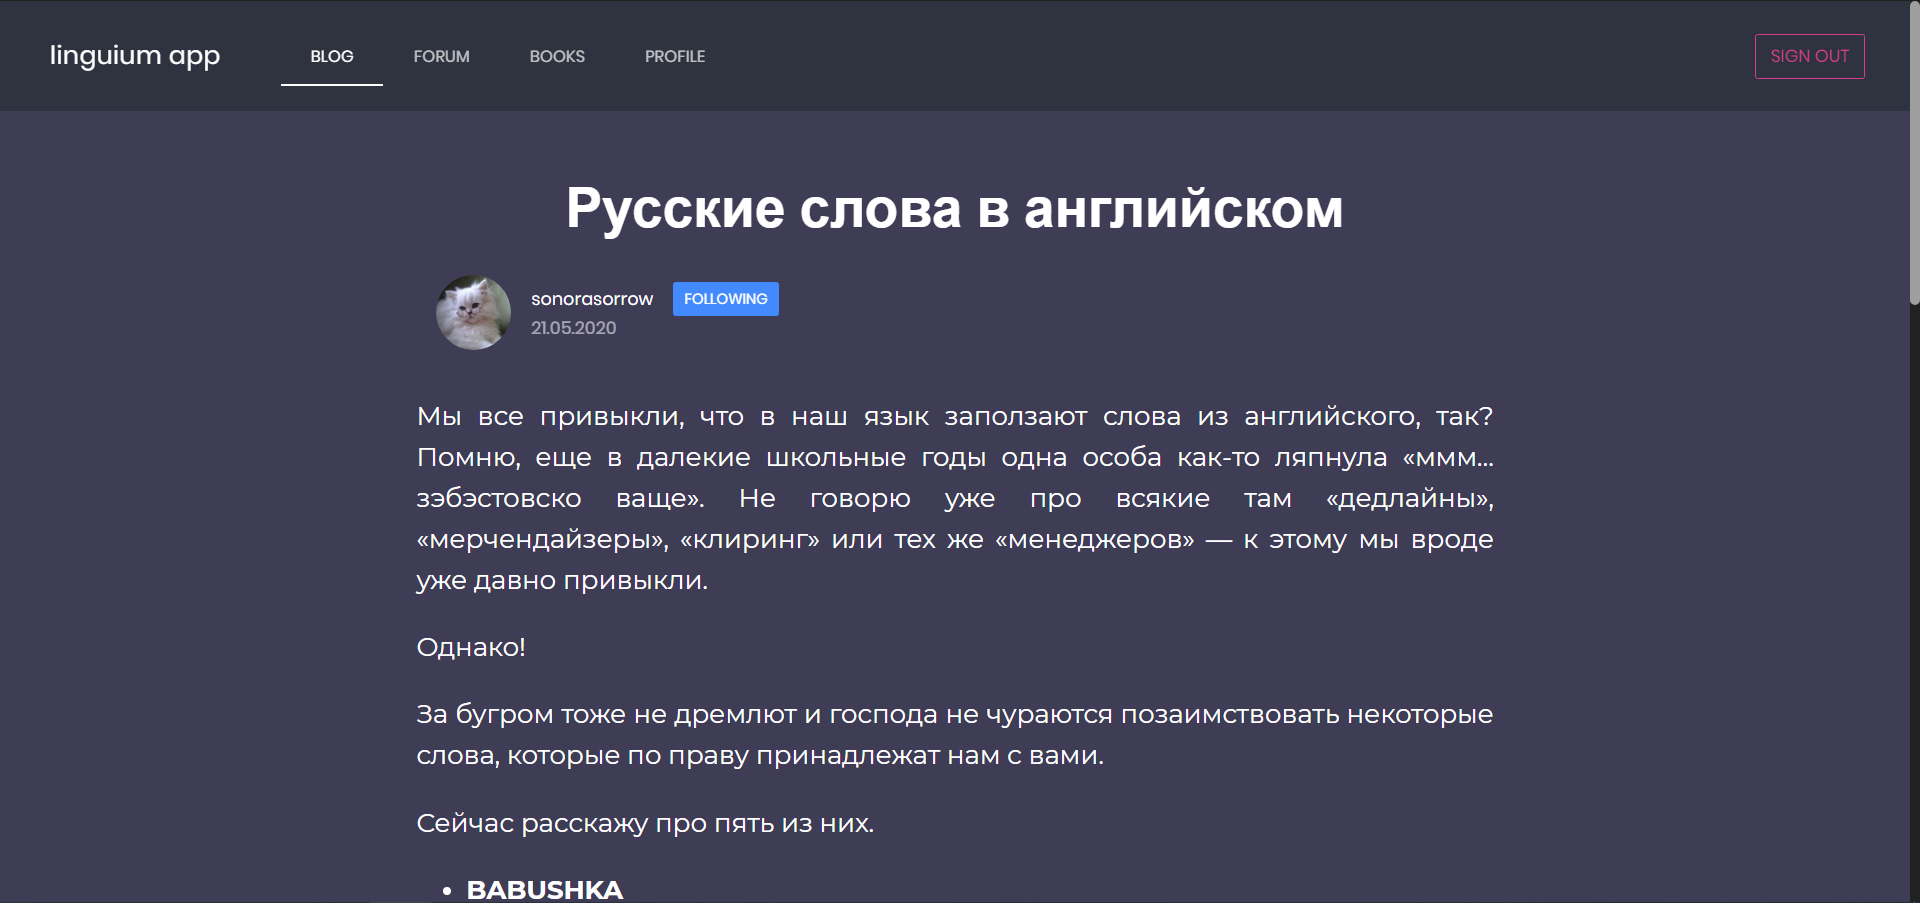
\includegraphics[width=\textwidth]{figures/articleitem}
	\caption{Содержимое конкретно взятой статьи}
	\label{fig:articleitem}
\end{figure}

\begin{figure}[h]
	\centering
	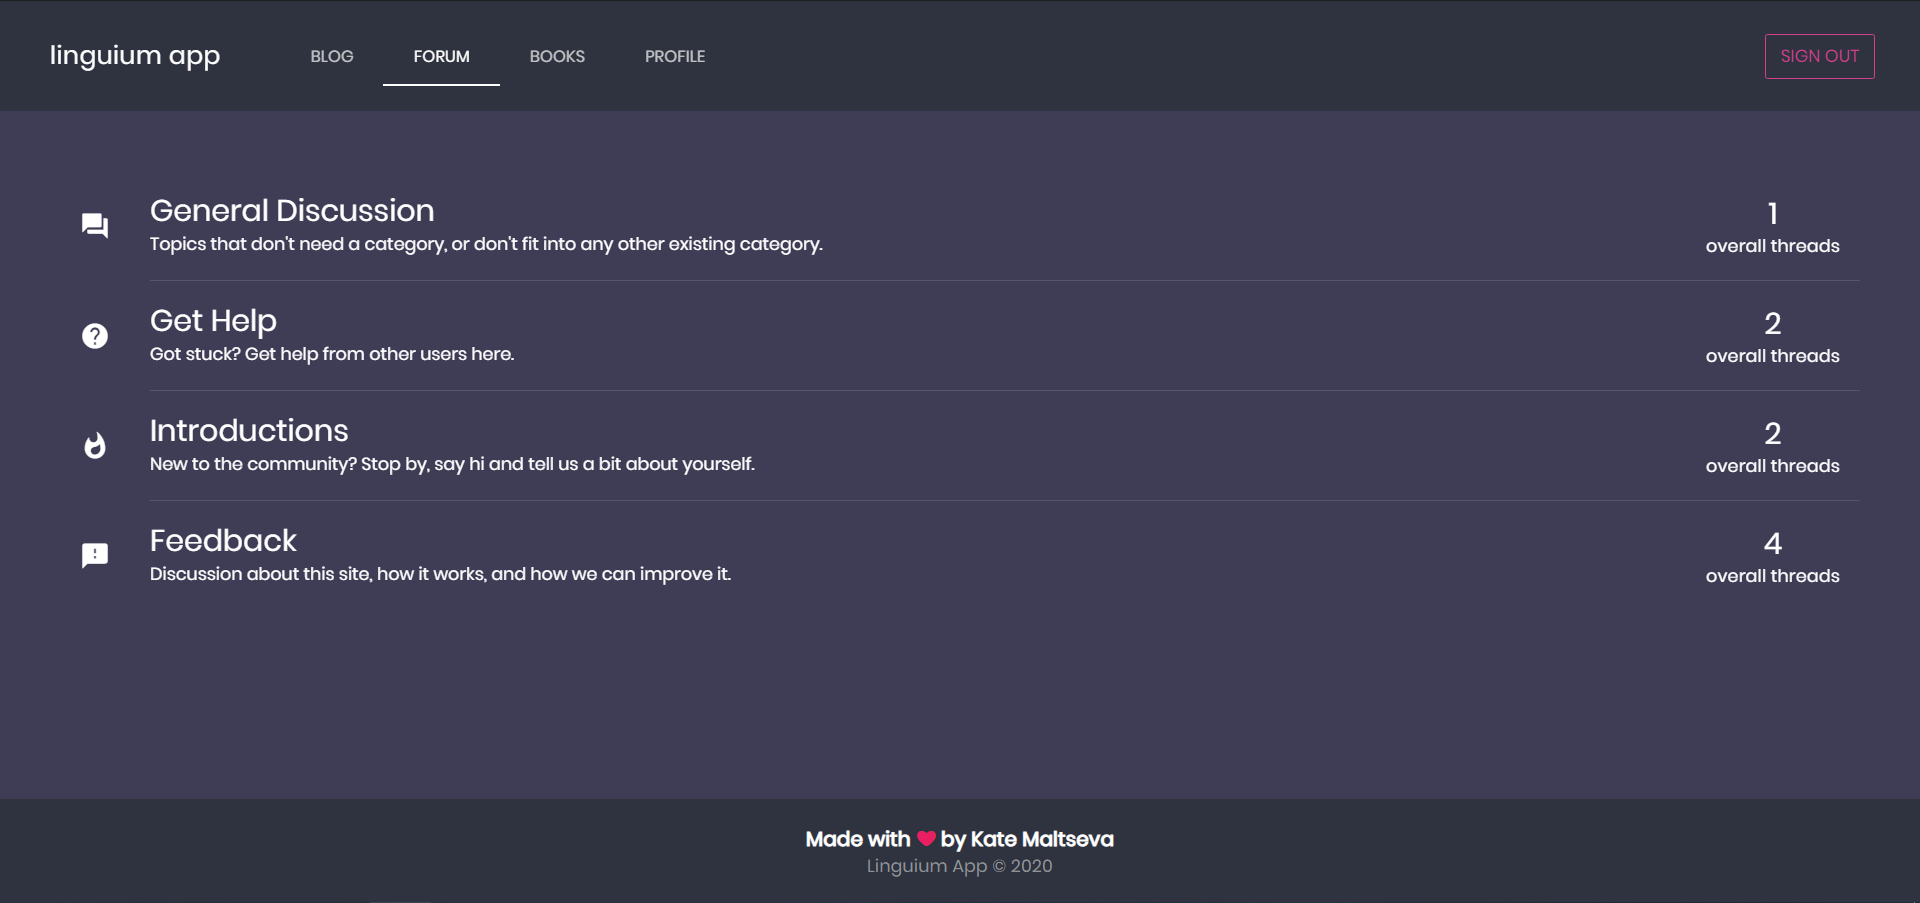
\includegraphics[width=\textwidth]{figures/forumlist}
	\caption{Форум: список всех доступных разделов и описание к ним}
	\label{fig:forumlist}
\end{figure}

\begin{figure}[h]
	\centering
	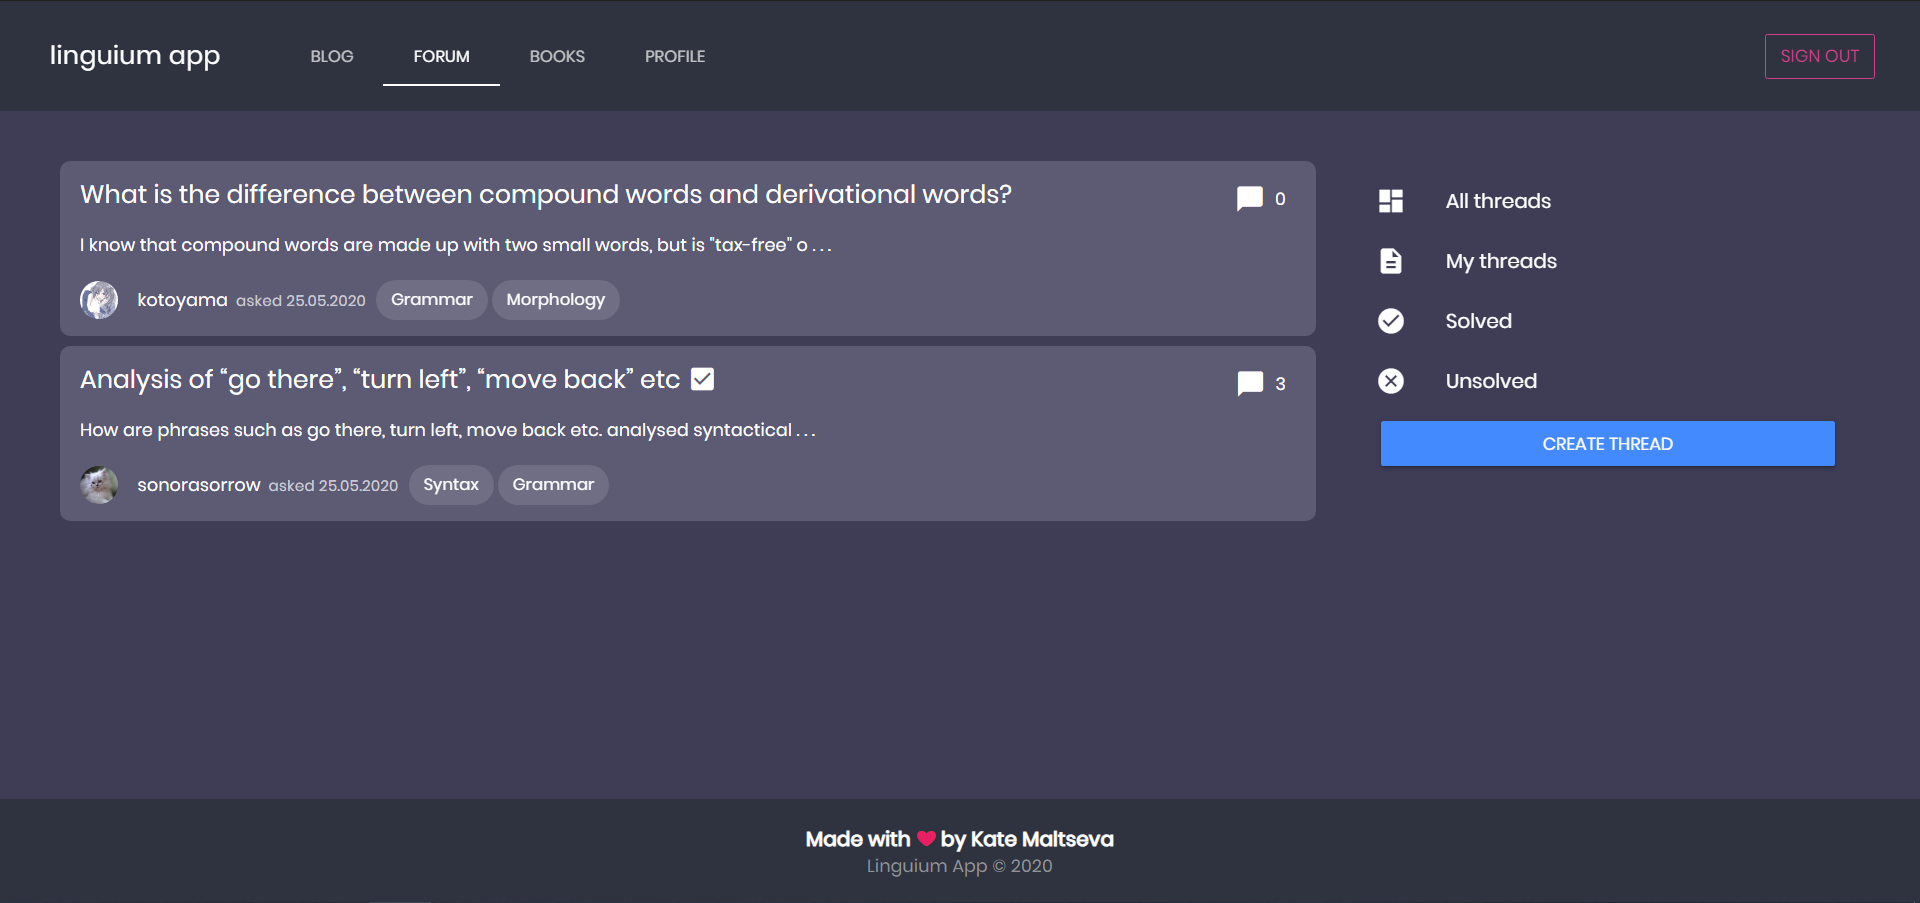
\includegraphics[width=\textwidth]{figures/topic}
	\caption{Список тредов к конкретно заданному разделу}
	\label{fig:topic}
\end{figure}

\begin{figure}[h]
	\centering
	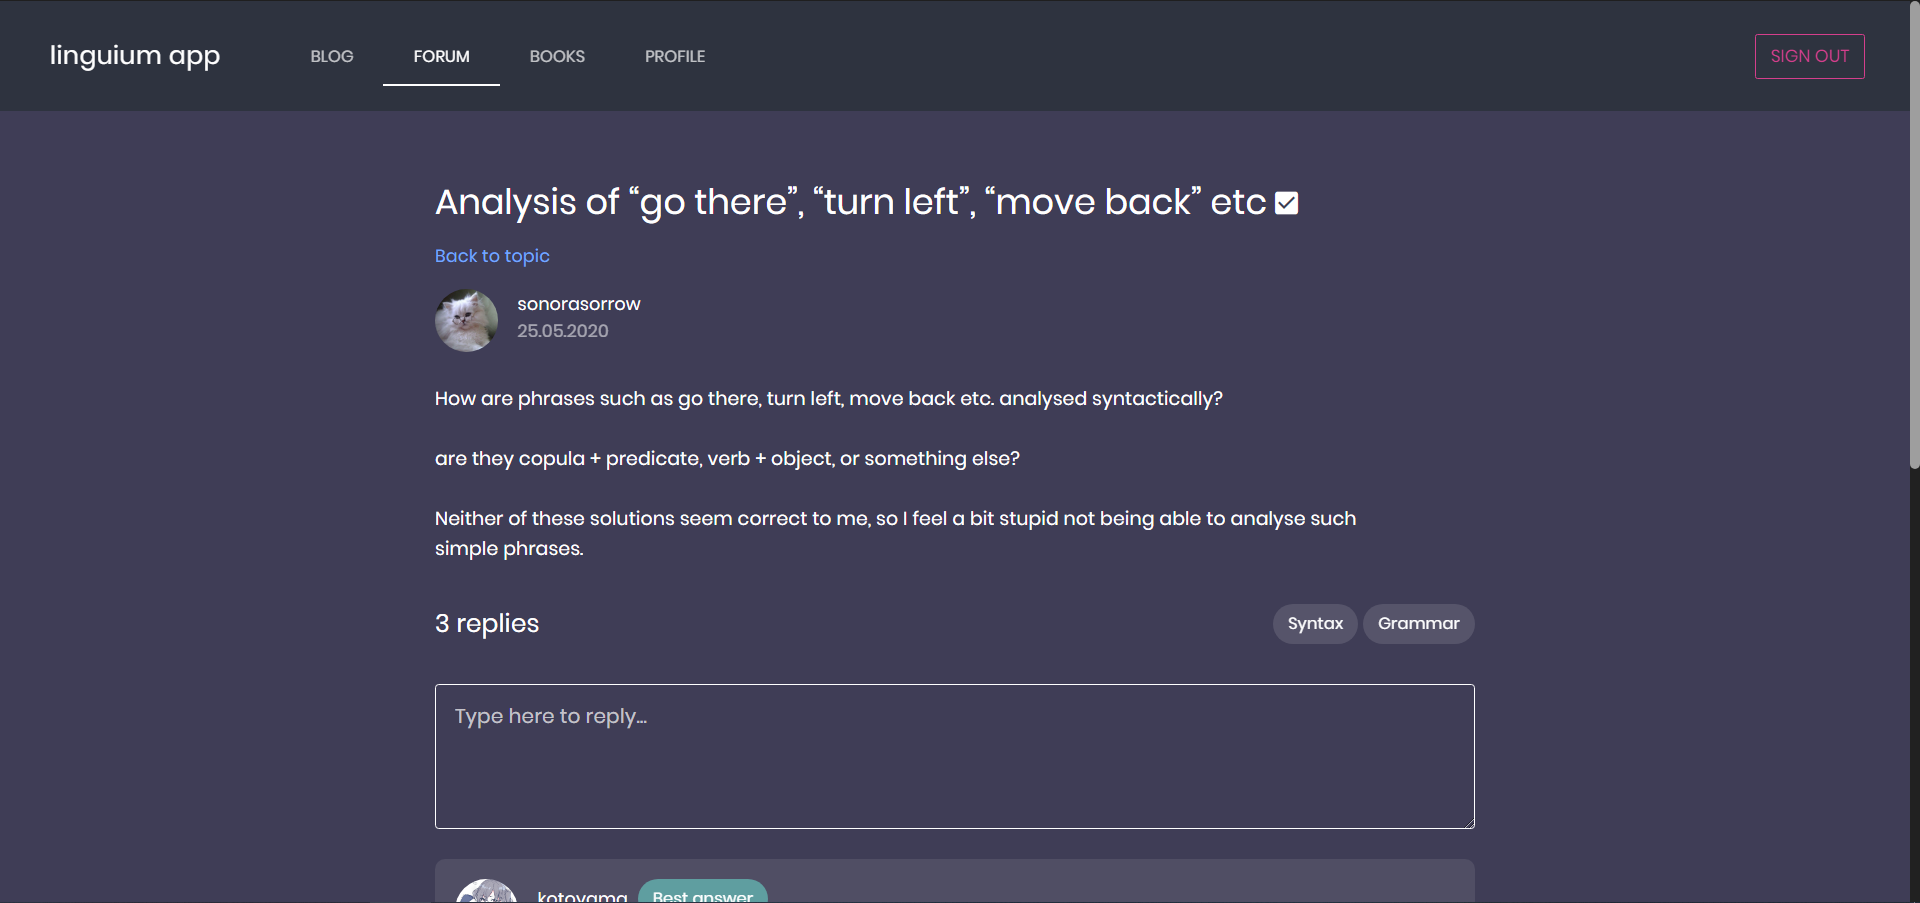
\includegraphics[width=\textwidth]{figures/thread}
	\caption{Содержимое конкретно заданного треда}
	\label{fig:thread}
\end{figure}

\begin{figure}[h]
	\centering
	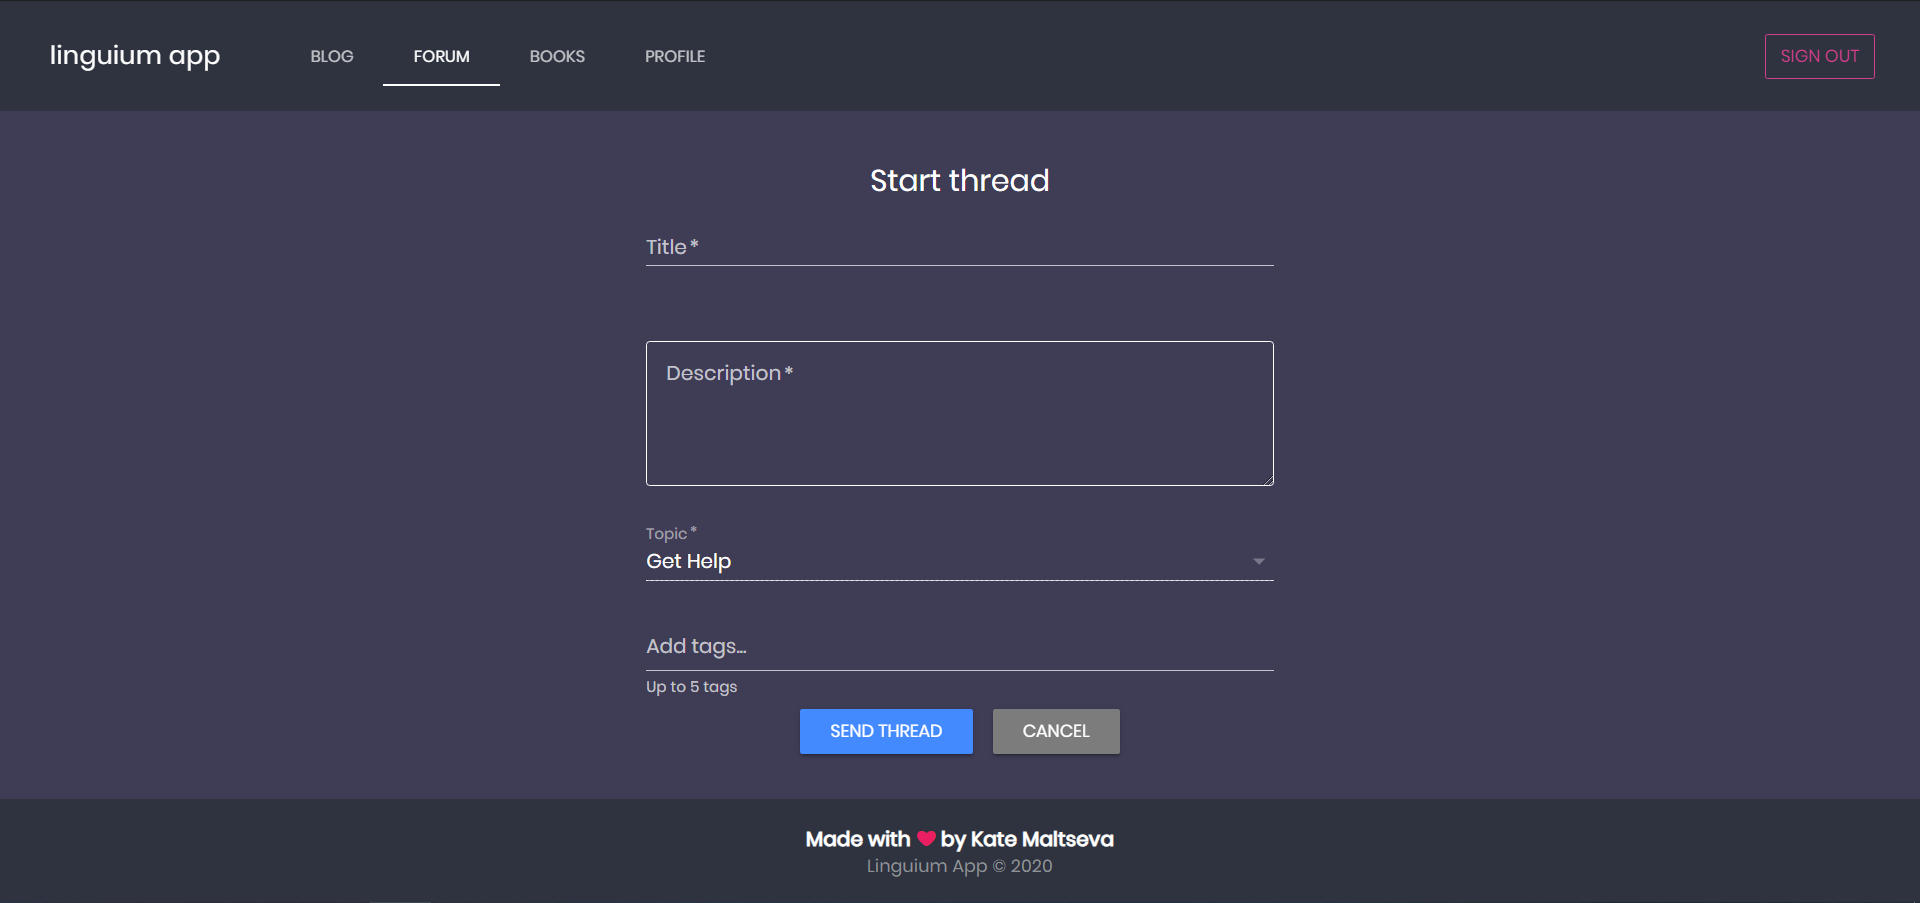
\includegraphics[width=\textwidth]{figures/createthread}
	\caption{Страница создания треда (страница для редакторования выглядит аналогичным образом)}
	\label{fig:createthread}
\end{figure}

\begin{figure}[h]
	\centering
	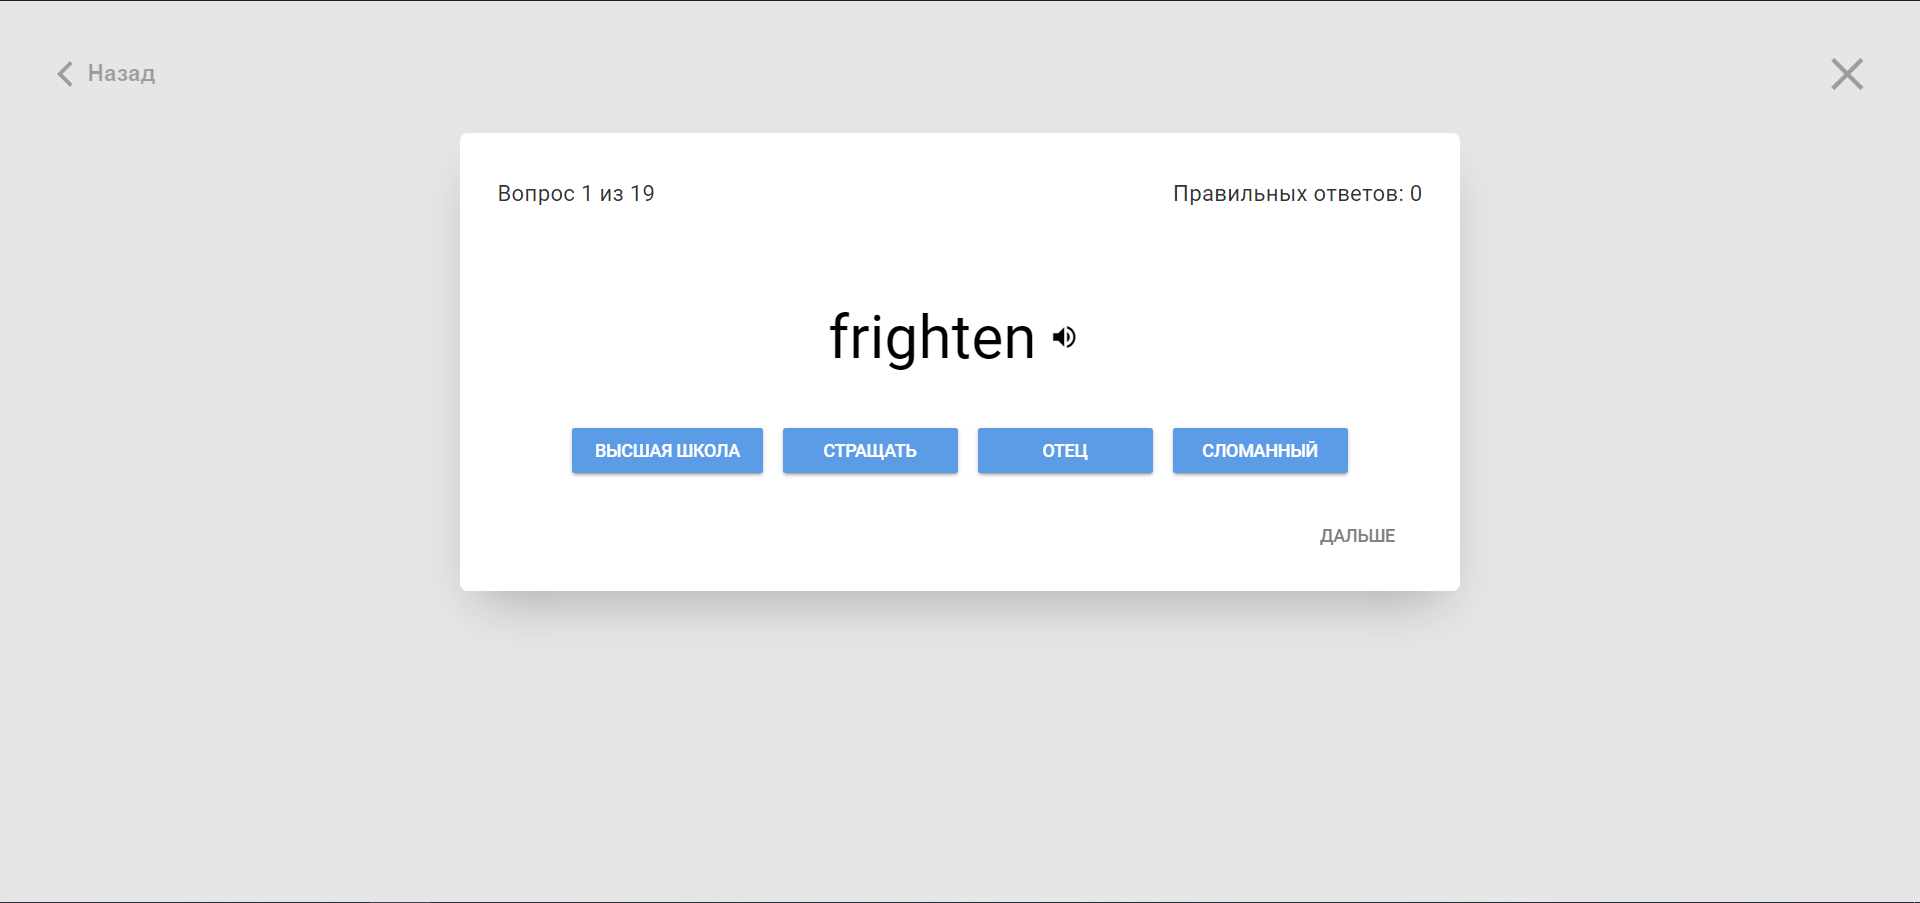
\includegraphics[width=\textwidth]{figures/trainer}
	\caption{Страница с тренажером для изучения слов}
	\label{fig:trainer}
\end{figure}

\begin{figure}[h]
	\centering
	
\includegraphics[width=\textwidth]{figures/404}
	\caption{Страница ошибки}
	\label{fig:404}
\end{figure}

%%% Local Variables: 
%%% mode: latex
%%% TeX-master: "rpz"
%%% End: 
